\section{Урвуу инженерчлэл: "Auftragsverwaltung" систем дэх зохиомжийн үлгэр загварууд}
Энэ хэсэгт Жава технологийг ашиглан хэрэгжүүлсэн бараа захиалгийг зохицуулах Герман нэршлийн конвенцтэй "Auftragsverwaltung" систем дээр урвуу инженерчлэлийн аргачлалаар програм хангамжийн зохиомжийн үлгэр загваруудыг уг системд хэрхэн ашигласан байгааг олж тогтооно.

\subsection{Системийн статик загвар}
Системийн классын диаграмыг гаргахын тулд Eclipse IDE дээрх PlantUML\footnote{https://plantuml.com/eclipse} програм хангамжийн багажыг ашигласан. Гэвч энэ багаж нь классууд хоорондын холбоосуудыг, тухайлбал бүрдмэл, нийлмэл зэрэг холбоог оновчтой гаргаж чадаагүй. Юуны түрүүнд энэ системийн нэршлийн конвенц нь Герман хэл дээр хийгдсэн учир тодорхой үгсийн Герман–Англи нэршлийн конвенцийг гаргах шаардлага үүссэн. Жишээ нь, "Auftragsverwaltung" нь "OrderManagement" буюу захиалгын удирдлага, "Auftrag" нь Order" буюу захиалга, "Kunde" нь "Customer" буюу харилцагч, "auftragLoeschen" нь "deleteOrder" буюу Order (Aufrag) классын устгагч гэх мэт. Хавсралт B хэсгээс эдгээр орчуулгыг харж болно.

Холбоосуудын төрлийг тодорхойлохын тулд класс тус бүрийн устгагчийн хэрэгжүүлэлтийг ажигласан. Жишээ нь, Order (Aufrag), OrderItem (Aufragsposition) классуудын хувьд Order классын объектийг устгах үед OrderItem классын объектуудаас бүрдсэн вектороор entfernenPos аргын тусламжтай гүйж устгаж байна. Харин Customer (Kunde) классын объектыг устгалгүй үлдээсэн байна. Иймд Order, OrderItem классууд хоорондоо нийлмэл холбоотой бол Order, Customer классууд хоорондоо бүрдмэл холбоотой гэж дүгнэлээ.
\begin{lstlisting}[language=Java, caption=Order классын устгагч auftragLoeschen, frame=single]
public boolean entfernenPos(Auftragsposition apos)
{
    boolean rc = apositionen.remove(apos);
    if (rc)
        this.aktualisieren();
    return rc;
}

public void auftragLoeschen()
{
    Iterator<Auftragsposition> positionen =
            apositionen.iterator();
    while (positionen.hasNext())
    {
        entfernenPos(positionen.next());
    }
}
\end{lstlisting}

Үүнтэй адилаар "Applicationlogic" багцын бүх классын нэрсийг жагсааж, тэдгээрийн хоорон -дын холбоосуудыг илрүүлсэн. Дараа нь, холбоосуудын төрлийг тодорхойлж, UML классын диаграмыг гаргасан. Үүний үр дүнг \ref{fig:diagram1} зурагт үзүүлэв. Мөн Item (Artikel) класс нь гадаад "Utility" багцаас (зураг \ref{fig:diagram4})\quad Money (Geld) классыг ашиглаж байгаа тул энэ холбоосыг харуу -лаагүй болно.

\begin{figure}
	\centering
	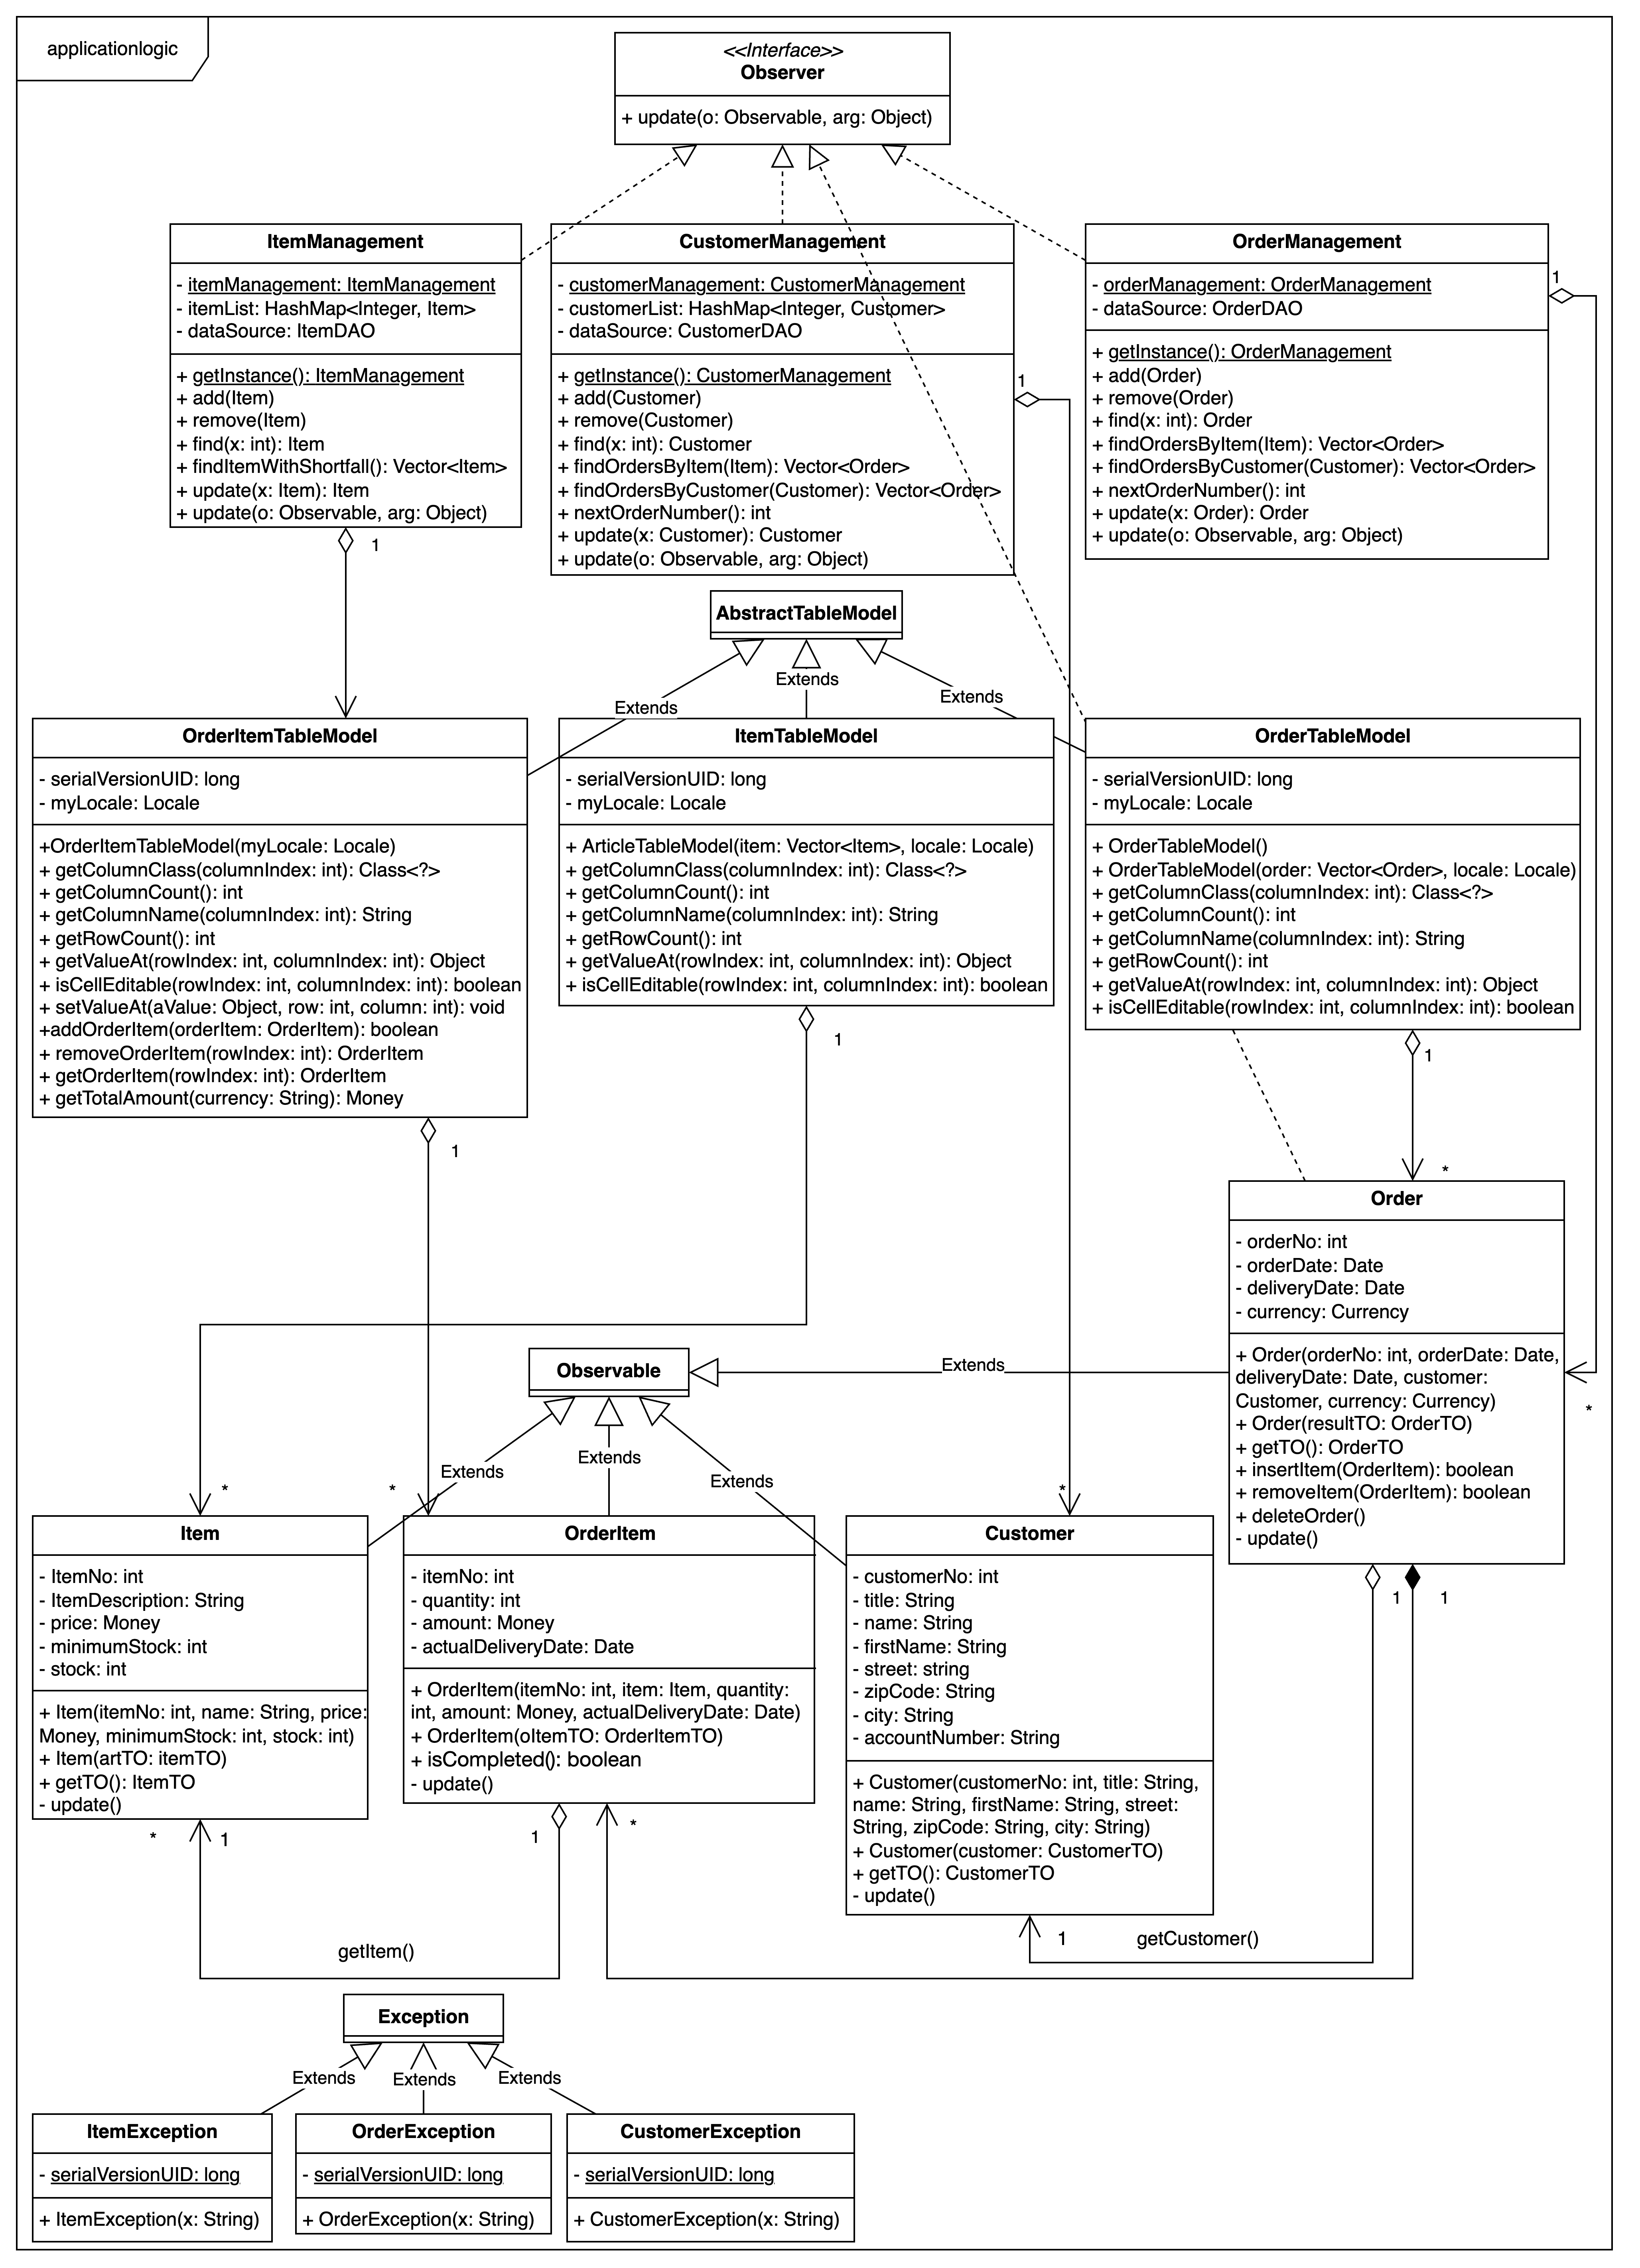
\includegraphics[width=15cm]{images/diagram1.png}
	\caption{"Applicationlogic" багцын классын диаграм}
	\label{fig:diagram1}
\end{figure}

\begin{figure}
	\centering
	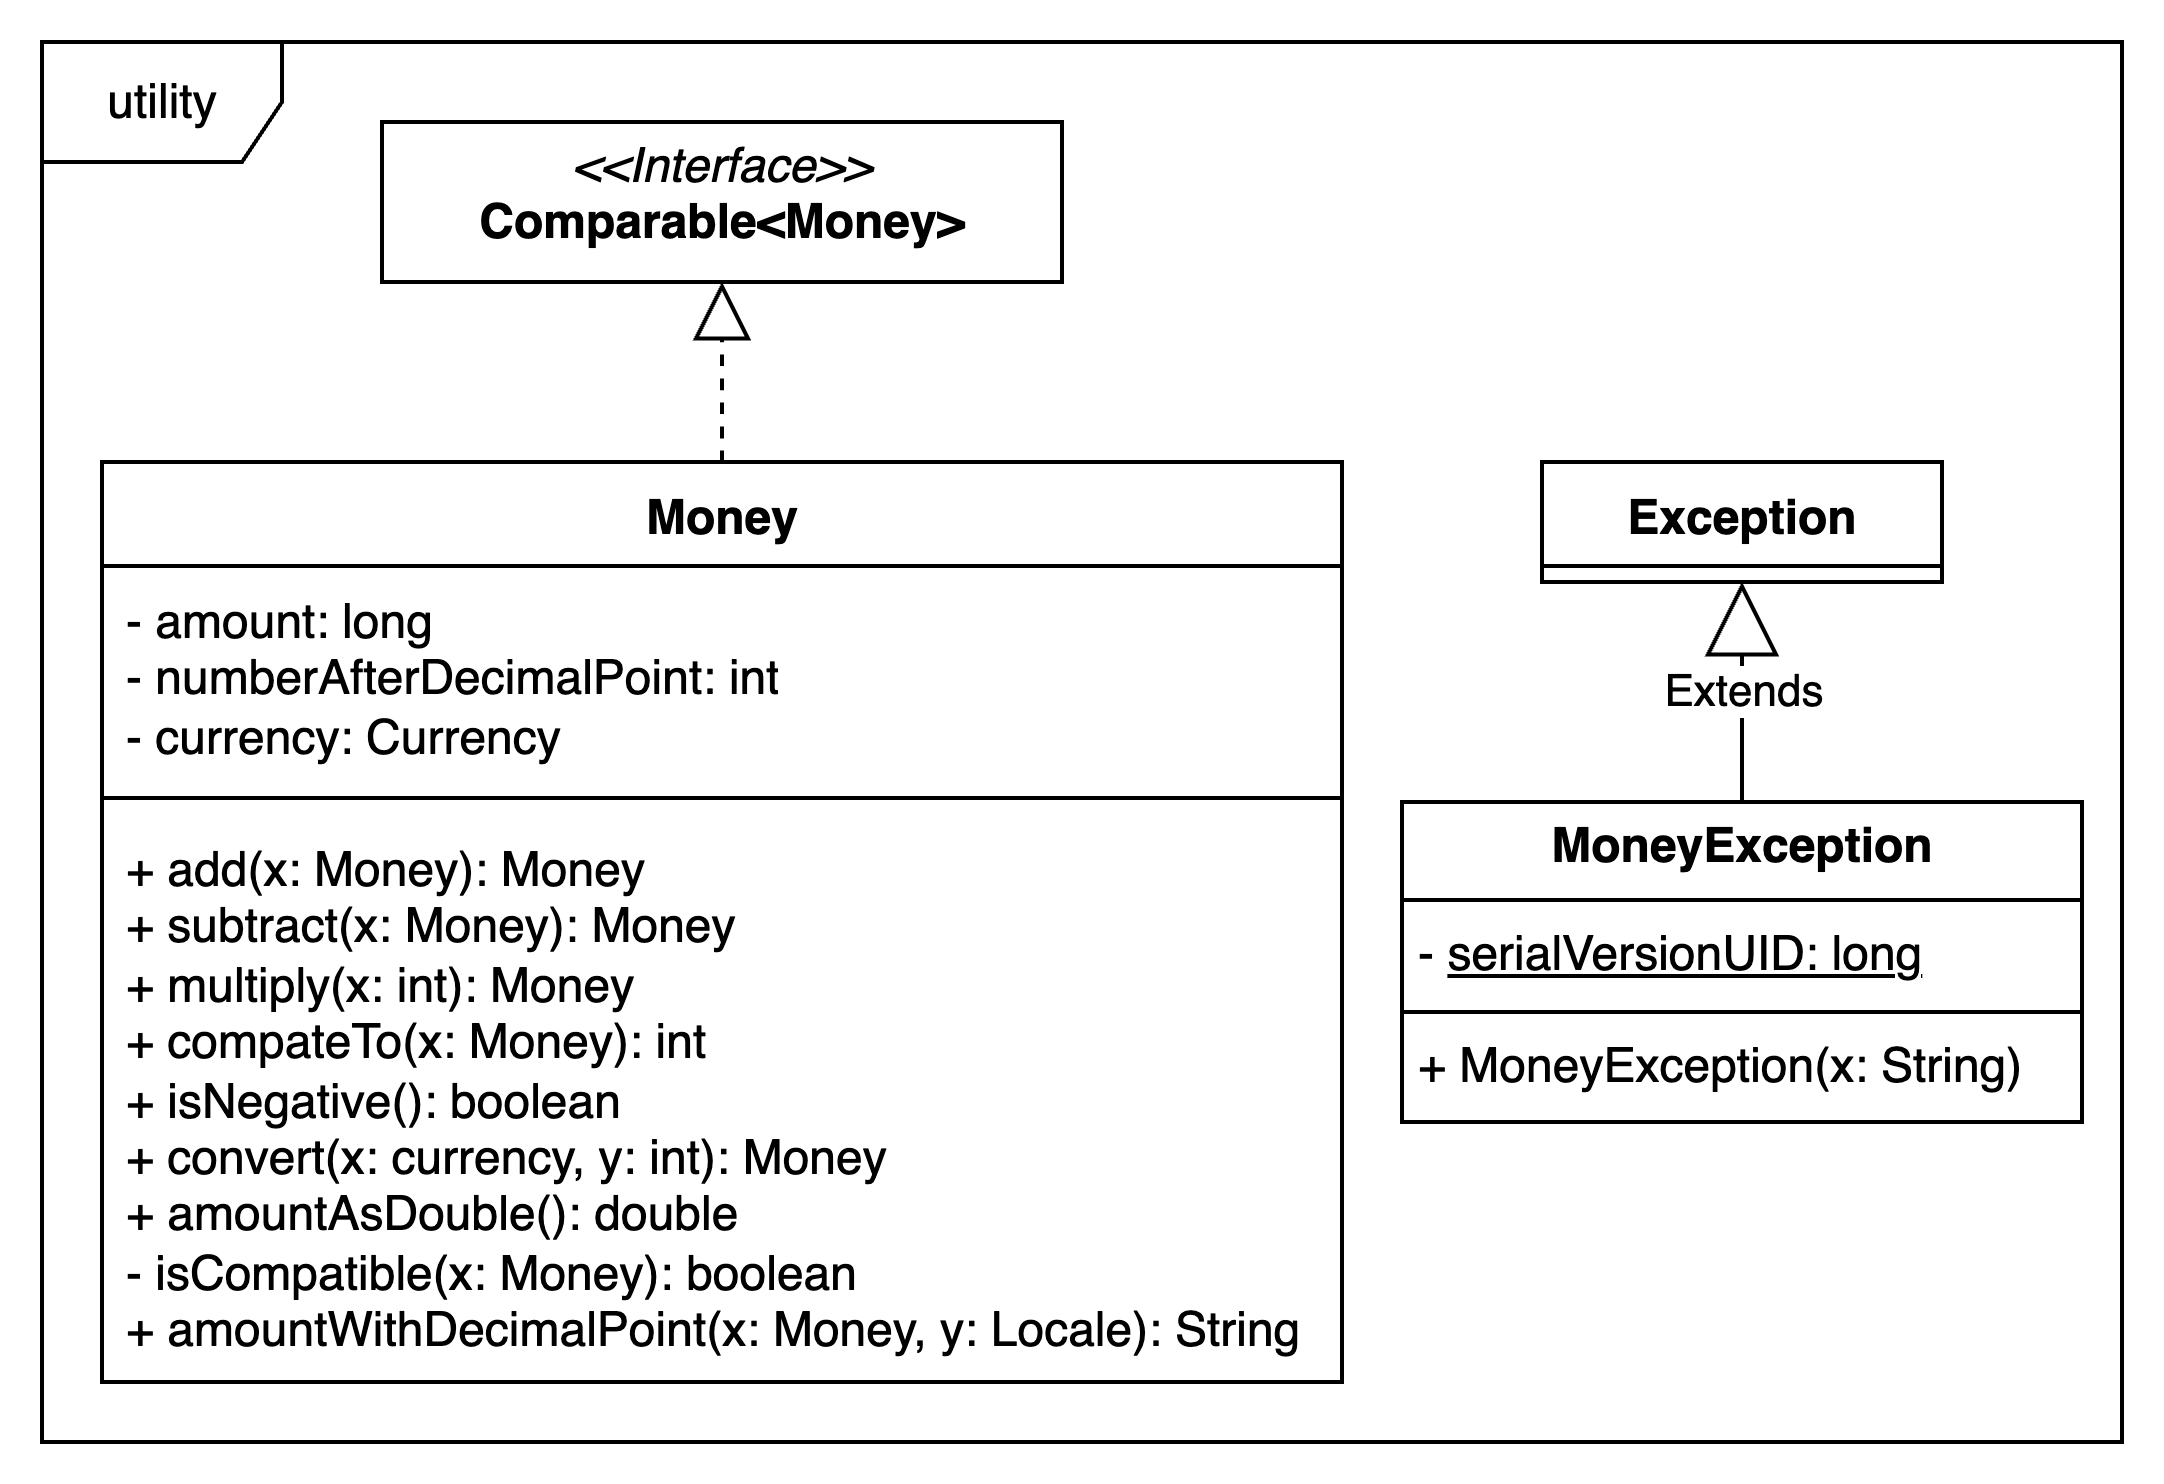
\includegraphics[width=10cm]{images/diagram4.png}
	\caption{"Utility" багцын классын диаграм}
	\label{fig:diagram4}
\end{figure}

\subsection{Системийн зохиомж}
Энэ хэсэгт "Auftragsverwaltung" системд илрүүлсэн гол зохиомжийн үлгэр загваруудын зорилго, хэрэглээ, бүтцийн элемент, өмнө тулгарч болох асуудал, үр дүн, жишээ код болон систем доторх бодит хэрэгжүүлэлтийг дэлгэрэнгүй авч үзнэ.

\subsubsection{"Iterator" үлгэр загвар}
Order классын бүх талбар, аргуудаар статик уншлага хийн \verb|apositionen.iterator()|,\\ \verb|while (positionen.hasNext())|,\verb| positionen.next()| мөрүүдийг тэмдэглэж үлгэр загварт заавал байх элементүүд кодод ямар хэлбэрээр илэрсэнг харлаа. Энд apositionen нь \textit{бүрдэл} болж, түүний \verb|iterator()| аргыг дуудаж байгаа нь "Iterator" интерфэйсийг ашиглаж буйг илтгэнэ. \verb|auftragLoeschen()| болон \verb|getAuftragssumme()| мэт аргуудын давталтын логикыг уншиж, хэрхэн давталт явдаг, давталтын үед ямар үйлдэл хийгдэхийг тодруулсан. Давталтын туршид бүрдлүүдтэй хэрхэн харьцаж байгааг анхааран харж, "concurrent modification"\footnote{Конкуррент програмчлалд өгөгдлийн бүтцийг өөр процесс эсвэл тредээр давтаж байх үед өөрчилсөн тохиолдолд "concurrent modification" үүсдэг. Энэ нь үнэн байхаа больсон өгөгдлийн бүтцээр гүйснээс үүдсэн урьдчилан таамаглах боломжгүй өгөгдлийн эвдрэл эсвэл "runtime error" алдааг үүсгэж болно.} зэрэг асуудал үүсэх эрсдлийг тооцсон. Дээрх ажиглалтаас үлгэр загварын шинж тэмдгүүд илэрсэн тул тухайн кодонд "Iterator" үлгэр загвар ашиглагдсан гэж тодорхойлсон. Энд apositionen нь \verb|Vector<Auftragsposition>| бөгөөд давталт хийхдээ \verb|apositionen.iterator()| ашиглагдаж байна. \verb|getAuftragssumme()| нь \verb|while(positionen.hasNext()){...positionen.next()...}| маягаар стандарт давталтыг ашиглан бүх Amount (Betrag) буюу үнийн дүнг олж байна. Энэ нь "Iterator" интерфэйсийн классик хэрэглээ юм.

\begin{lstlisting}[language=Java, caption=Order классын арга getAuftragssumme, frame=single]
  public Geld getAuftragssumme()
  {
    Iterator<Auftragsposition> positionen =
        apositionen.iterator();
    Geld ergebnis = new Geld(0, 0, waehrung);
    if (positionen.hasNext())
      ergebnis = new Geld(positionen.next().getBetrag());
    while (positionen.hasNext())
    {
      ergebnis.addieren(positionen.next().getBetrag());
    }
    return ergebnis;
  }
\end{lstlisting}

\subsubsection{"Singleton" үлгэр загвар}
OrderManagement классын статик талбар дээр шууд \verb|new Auftragsverwaltung()| дуудаж байгаа нь "eager initialization"\footnote{"Eager initialization" нь програмчлалын стратеги бөгөөд объект эсвэл нөөцийг анх ашиглахыг хүсэх хүртэл хүлээх биш, агуулагдсан класс нь ачаалагдсан даруйд үүсгэгддэг.} бөгөөд тредүүдэд аюулгүй байдаг боловч хэзээ ч ашиглагдахгүй объект байгуулагдах эрсдэлтэй. Мөн \verb|DAOFactory.getInstance()| гэх мэт глобал хандалтын цэгүүдийг ажиглалаа.   Класс нь өөрөө "Observer"-ыг хэрэгжүүлж, менежментийн үүрэг гүйцэт- гэж байгаа ч байгуулагчийг private гэж огт заагаагүй тул шинэ Auftragsverwaltung объектыг байгуулж параллел объект үүсгэх эрсдэлтэй. \verb|hinzufuegen()| дотор \verb|auf.addObserver(this)| гэж байгаа нь Singleton объект өөрөө Observable объектын өөрчлөлтийг хүлээн авч DAO-руу update илгээж байна. Энэ бүх ажиглалтуудаас жинхэнэ "Singleton" үлгэр загварыг ашиглаагүй гэж дүгнэлээ. Харин өөр нэг үлгэр загварыг олсон нь "Observer" юм. Үүнийг дараагийн хэсэгт тайлбарлав.
\begin{lstlisting}[language=Java, caption=OrderManagement классын арга hinzufuegen, frame=single]
  private static Auftragsverwaltung eineAuftragsverwaltung = new Auftragsverwaltung();

  public void hinzufuegen(Auftrag auf)
      throws AuftragException
  {
    int auftragsnr = auf.getAuftragsnr();
    try {
      if (datenquelle.read(auftragsnr) != null)
        throw new AuftragException(
            "Auftrag mit dieser Nummer ist schon vorhanden");
      datenquelle.create(auf.getTO());
      auf.addObserver(this);
    } catch (Exception ex)
    {
      throw new AuftragException("Auftrag " + auftragsnr
          + " konnte nicht gespeichert werden!");
    }
  }
\end{lstlisting}

\subsubsection{"Observer" үлгэр загвар}

OrderManagement классын \verb|hinzufuegen()| дотор \verb|auf.addObserver(this)| гэж байгаа нь Singleton объект өөрөө Observable объектын өөрчлөлтийг хүлээн авч DAO-руу update илгээж байна. Үүнийг ажигласнаар "Observer" үлгэр загвар ашиглагдсан гэж дүгнэлээ. Үлгэр загварын бүтэц, оролцогчдыг \ref{fig:observer} диаграммаар үзүүлэв. Үүнд:

% \begin{lstlisting}[language=Java, caption=, frame=single]
% \end{lstlisting}


% \begin{lstlisting}[language=Java, caption=, frame=single]
% \end{lstlisting}


% 5.3 Singleton Pattern
% Intent: Тухайн классийн ганцхан экземпляр (instance) байдаг гэдгийг баталгаажуулж, олон удаа үүсэхээс хамгаалдаг.
% Applicability:
% •	Нэглхэн resource (DB холболт, конфигурацийн тохиргоо) хуваарилах шаардлагатай.
% Participants:
% •	Singleton Class: DBConnection, Datenquelle
% Consequences:
% •	Global access point үүснэ.
% •	Тестлэхэд заримдаа бэрхшээл үүсгэж, dependency injection-тэй зэрэгцүүлэн ашиглахгүй болбол.
% Жишээ код:
% public class DBConnection {
%     private static volatile DBConnection instance;
%     private Connection conn;
%     private DBConnection() { /* connect */ }
%     public static DBConnection getInstance() {
%         if (instance == null) {
%             synchronized(DBConnection.class) {
%                 if (instance == null) instance = new DBConnection();
%             }
%         }
%         return instance;
%     }
% }
 
% 5.4 Composite Pattern
% Intent: Бүхэл–хэсэг (whole–part) харилцааг нэгтгэн, нэг объект ба хэд хэдэн ижил төрлийн объектын мод бүтэцтэй зохион байгуулалт бий болгодог.
% Applicability:
% •	Нэг Order нь олон OrderItem агуулсан тохиолдолд.
% Participants:
% •	Component: AuftragComponent (interface)
% •	Leaf: Auftragsposition
% •	Composite: Auftrag (ихээр OrderItem-уудыг барьдаг)
% Consequences:
% •	Дүрслэл тодорхой, ижил үйлдэлд ижил интерфейс ашиглагдана.
% •	Доторх мод бүтцийн гүнзгий давталт хэрэгтэй бол гүйцэтгэл саатах магадлалтай.
% Жишээ код:
% interface AuftragComponent { void print(); }
% class Auftragsposition implements AuftragComponent { public void print() { ... } }
% class Auftrag implements AuftragComponent {
%     private List<Auftragsposition> items;
%     public void add(Auftragsposition p) { items.add(p); }
%     public void print() { for (Auftragsposition p: items) p.print(); }
% }
 
% 5.5 MVC (Model–View–Controller) Pattern
% Intent: Хэрэглэгчийн интерфейс (View), бизнес логик (Model), үйлдлийн урсгал (Controller)-ыг тусад нь тусгаарлаж, харилцан нөлөөллийг багасгах.
% Applicability:
% •	UI бүхий desktop, web эсвэл mobile аппликейшн хөгжүүлэхдээ.
% Participants & Flow:
% 1.	Model: Kunde, Artikel, Auftrag — өгөгдлийн асуудлыг илэрхийлэх.
% 2.	View: BenutzerGUI — хэрэглэгчид харагдах интерфейс.
% 3.	Controller: OrderController — View-аас ирсэн үйлдлийг хүлээн авч Model дээр үйлдэл гүйцэтгэнэ.
% Жишээ диаграмм (high-level):
% [User Action] -> Controller -> Model -> View Update
% Жишээ код:
% public class OrderController {
%     private OrderManager model;
%     private OrderView view;
%     public void handleAddOrder(Auftrag o) {
%         model.addOrder(o);
%         view.refresh(model.getOrders());
%     }
% }
 
% 5.6 Observer Pattern
% Intent: Subject (Observable) болон түүний харагч объектууд (Observers) хоорондын уялдааг тодорхой болгож, Subject-ийн төлөв (state) өөрчлөгдөх бүрт харагчид автоматаар мэдээлэл өгч шинэчлэгддэг боломжийг олгоно.
% Applicability:
% •	Domain Model дэх объектоудын статус өөрчлөгдөхөд бусад бүрэлдэхүүн (UI TableModels, Verwaltung classes, ReportGenerator) автоматаар шинэчлэгдэх шаардлагатай.
% •	Тасралтгүй өгөгдлийн урсгал ба UI синхронизац (жишээ нь, шинэ Order нэмэгдэх, OrderItem-уудын тоо эсвэл утга өөрчлөгдөх үед хүснэгт автоматаар шинэчлэгдэх) хэрэгтэй тохиолдолд.
% Structure (UML-д илэрсэнээр):
%             +--------------+            +---------------------+
%             |  Observable  |            |     Observer        |
%             +--------------+            +---------------------+
%             | +addObserver()|<>-------->*| +update(Observable, Object)|
%             | +notifyObservers()|        +---------------------+
%             +--------------+
%                   ^   ^
%                   |   |
%   +---------------+   +-------------------+
%   |                                    |
% +--------+                         +-------------+
% | Kunde  |                         | Auftragsposition |
% +--------+          ...            +-------------+
%   ^                                         ^
%   |                                         |
% +---------+                          +--------------+
% | Auftrag |                          | Artikelverwaltung |
% +---------+                          +--------------+
% •	Domain Objects (Subjects): Kunde, Auftrag, Auftragsposition, Artikel зэрэг ангиуд нь Observable-ээс өвлөн авч, өөрийн төлөв өөрчлөгдөх мөчид notifyObservers()-ыг дуудаж бүх бүртгэлтэй Observer-уудыг мэдэгддэг.
% •	Verwaltung Classes (Observers): Kundenverwaltung, Auftragsverwaltung, Artikelverwaltung зэрэг нь Observer интерфейсийг хэрэгжүүлэн, update() аргаар domain объектоос ирсэн өөрчлөлт, шинэчлэлтийг хүлээн авдаг.
% •	TableModel Classes (UI Observers): ArtikelTableModel, AuftragTableModel, AuftragspositionTableModel зэрэг нь мөн Observer интерфейсийг хэрэгжүүлэн, update() дотор fireTableDataChanged() эсвэл тухайн мөр/баганыг шинэчлэх аргуудыг дуудаж хэрэглэгчийн дэлгэцийн хүснэгтийг автоматаар шинэчилдэг.
% Collaboration:
% 1.	Domain объектын setXxx(...) эсвэл бизнесийн үйлдлээр (addOrder, removePosition, updatePrice гэх мэт) төлөв нь өөрчлөгдөх үед aktualisieren() дотор notifyObservers(this, context) дуудаж өгөгдлийг тараана.
% 2.	Бүртгэгдсэн Verwaltung ба TableModel объектуудын update(Observable o, Object arg) дотор ирсэн мэдээллийг боловсруулан бизнес давхарга болон UI-г шинэчилнэ.
% Consequences:
% •	UI ба Domain Logic хоорондох хатуурсан coupling-ийг багасгаж, хоёр талын автомат синхронизацад дэмжлэг үзүүлнэ.
% •	Java-ийн хуучин Observable/Observer ашигласан тул дээд төвшний flexibility-ийн хувьд зарим хязгаарлалттай (abstract class тул олон өвлөн авалт боломжгүй гэх мэт).
% •	Их олон объект холбогдсоны улмаас notification avalanche үүсэх, performance буурах эрсдэлтэй.
% Жишээ код:
% public class Auftrag extends Observable {
%     public void setLieferdatum(LocalDate date) {
%         this.lieferdatum = date;
%         aktualisieren(); // дотор нь notifyObservers(this)
%     }
% }

% public class AuftragTableModel extends AbstractTableModel implements Observer {
%     public void update(Observable o, Object arg) {
%         // шинэчлэгдсэн өгөгдлийг авсаны дараа хүснэгтээ шинэчилнэ
%         fireTableDataChanged();
%     }
% }

% public class Auftragsverwaltung implements Observer {
%     public void update(Observable o, Object arg) {
%         // бизнес давхарга дахь internal collection-ээ шинэчилнэ
%     }
% }
% System Usage Highlights:
% •	Flexible Event-Driven Архитектур: Системийн бүх чухал domain объектууд (Kunde, Artikel, Auftrag, Auftragsposition) нь Observable-ээс өвлөх замаар үзэгдлийн (event) төв болсон.
% •	Автомат UI Refresh: UI TableModel-ууд Observer-уудын хувьд табыг автоматаар шинэчлэн үзүүлдэг.
% •	Verwaltung Coordination: *verwaltung класс бүр domain объект болгон өөрийн collection-руу дахин оруулан, төвлөрсөн менежмент хийдэг.


% \begin{figure}
% 	\centering
% 	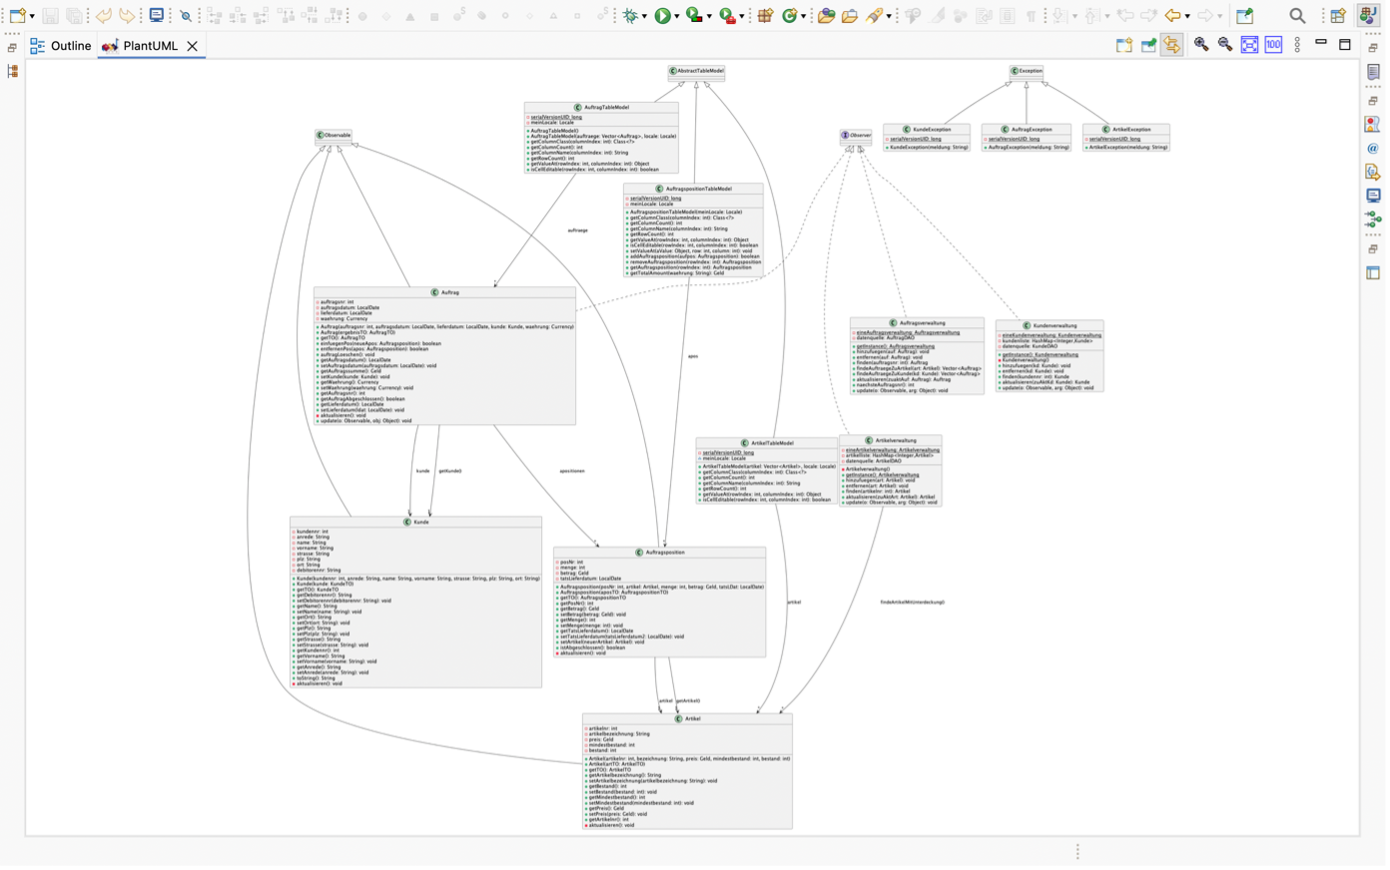
\includegraphics[width=15cm]{images/plantuml.png}
% 	\caption{UML багажаар үүсгэсэн "Applicationlogic" багцын классын диаграм}
% 	\label{fig:hhe}
% \end{figure}

\subsubsection{DAO (Data Access Object) үлгэр загвар}
Intent: Бизнес логик болон өгөгдлийн сан (database) хоорондох харилцааг салгаж, өгөгдлийн хандалтын кодыг төвлөрүүлдэг. Ингэснээр өгөгдлийн сангийн төрөл, схем өөрчлөгдөхөд бусад давхаргаас хамааралгүйгээр шинэчлэлт хийх боломжтой.
Applicability:
Өгөгдлийн сан, файлын систем, REST үйлчилгээ болон бусад I/O үйлдлүүдтэй тухайн давхаргын кодыг багцлах шаардлагатай үед.
Олон бизнес обьект өгөгдлийн үйлдэл хийх үед давталт, дубликацыг багасгах шаардлагатай бол.
Participants:
DAO Interface: SqlDAO<T> — нийтлэг өгөгдөл унших, бичих аргатай.
Concrete DAO: ArtikelDAO, KundeDAO, AuftragDAO — хүссэн хүснэгтийн өргөтгөл.
Model: Artikel, Kunde, Auftrag классууд.
Collaboration:
Business логик DAO interface-ээр дамжин өгөгдөл авах/хадгална.
Concrete DAO-ууд өгөгдлийн сангийн SQL query-үүдийг гүйцэтгэнэ.
Consequences:
Давхаргын тусгаарлалт сайжирна.
Тестлэхэд mock DAO ашиглах замаар өгөгдлийн сангүйгээр unit тест бичиж болно.
Өгөгдлийн сангийн холболт өөрчлөгдөхөд DAO давхаргыг л шинэчлэхэд хангалттай.
Жишээ код:

\begin{lstlisting}
\end{lstlisting}